\documentclass{standalone}
\usepackage{tikz}
\usetikzlibrary{patterns, positioning}
\usetikzlibrary{shapes.misc}
\usepackage[outline]{contour}
\contourlength{1.5pt} 


\begin{document}
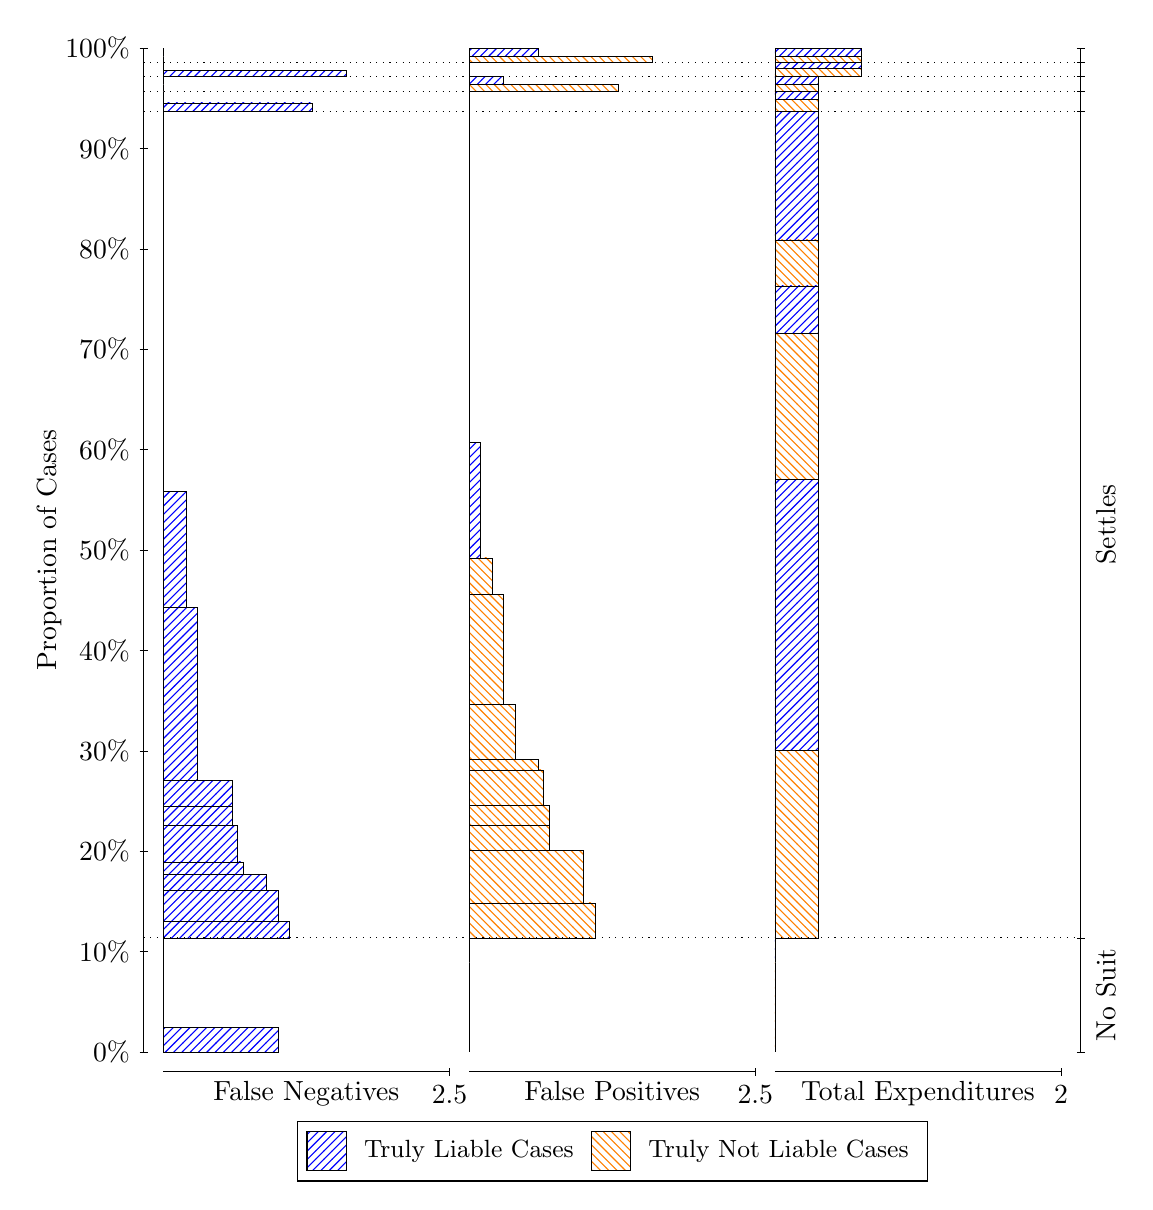
\begin{tikzpicture}
\draw[black, very thin] (1.5,1.75) -- (1.5,14.5);
\node[rotate=90, text=black, anchor=center] at (0.3, 8.125) {Proportion of Cases};
\draw[black, very thin] (1.45,1.75) -- (1.55,1.75);
\node[text=black, anchor=east] at (1.45, 1.75) {0\%};
\draw[black, very thin] (1.45,3.025) -- (1.55,3.025);
\node[text=black, anchor=east] at (1.45, 3.025) {10\%};
\draw[black, very thin] (1.45,4.3) -- (1.55,4.3);
\node[text=black, anchor=east] at (1.45, 4.3) {20\%};
\draw[black, very thin] (1.45,5.575) -- (1.55,5.575);
\node[text=black, anchor=east] at (1.45, 5.575) {30\%};
\draw[black, very thin] (1.45,6.85) -- (1.55,6.85);
\node[text=black, anchor=east] at (1.45, 6.85) {40\%};
\draw[black, very thin] (1.45,8.125) -- (1.55,8.125);
\node[text=black, anchor=east] at (1.45, 8.125) {50\%};
\draw[black, very thin] (1.45,9.4) -- (1.55,9.4);
\node[text=black, anchor=east] at (1.45, 9.4) {60\%};
\draw[black, very thin] (1.45,10.675) -- (1.55,10.675);
\node[text=black, anchor=east] at (1.45, 10.675) {70\%};
\draw[black, very thin] (1.45,11.95) -- (1.55,11.95);
\node[text=black, anchor=east] at (1.45, 11.95) {80\%};
\draw[black, very thin] (1.45,13.225) -- (1.55,13.225);
\node[text=black, anchor=east] at (1.45, 13.225) {90\%};
\draw[black, very thin] (1.45,14.5) -- (1.55,14.5);
\node[text=black, anchor=east] at (1.45, 14.5) {100\%};

\draw[black, very thin] (13.4,1.75) -- (13.4,14.5);
\draw[black, very thin] (13.35,1.75) -- (13.45,1.75);
\node[anchor=west] at (13.35, 1.75) {};
\draw[black, very thin] (13.35,3.2) -- (13.45,3.2);
\node[anchor=west] at (13.35, 3.2) {};
\draw[black, very thin] (13.35,13.695) -- (13.45,13.695);
\node[anchor=west] at (13.35, 13.695) {};
\draw[black, very thin] (13.35,13.95) -- (13.45,13.95);
\node[anchor=west] at (13.35, 13.95) {};
\draw[black, very thin] (13.35,14.14) -- (13.45,14.14);
\node[anchor=west] at (13.35, 14.14) {};
\draw[black, very thin] (13.35,14.321) -- (13.45,14.321);
\node[anchor=west] at (13.35, 14.321) {};
\draw[black, very thin] (13.35,14.5) -- (13.45,14.5);
\node[anchor=west] at (13.35, 14.5) {};

\draw[black, very thin, pattern color=blue, pattern=north east lines] (1.75,1.75) rectangle (3.2033,2.0609);
\draw[black, very thin, pattern color=orange, pattern=north west lines] (1.75,2.0609) rectangle (1.75,3.2);
\draw[black, very thin, pattern color=blue, pattern=north east lines] (1.75,3.2) rectangle (3.3487,3.4038);
\draw[black, very thin, pattern color=blue, pattern=north east lines] (1.75,3.4038) rectangle (3.2033,3.8018);
\draw[black, very thin, pattern color=blue, pattern=north east lines] (1.75,3.8018) rectangle (3.058,4.0015);
\draw[black, very thin, pattern color=blue, pattern=north east lines] (1.75,4.0015) rectangle (2.7673,4.164);
\draw[black, very thin, pattern color=blue, pattern=north east lines] (1.75,4.164) rectangle (2.6947,4.6293);
\draw[black, very thin, pattern color=blue, pattern=north east lines] (1.75,4.6293) rectangle (2.622,4.8766);
\draw[black, very thin, pattern color=blue, pattern=north east lines] (1.75,4.8766) rectangle (2.622,5.2032);
\draw[black, very thin, pattern color=blue, pattern=north east lines] (1.75,5.2032) rectangle (2.186,7.4002);
\draw[black, very thin, pattern color=blue, pattern=north east lines] (1.75,7.4002) rectangle (2.0407,8.8712);
\draw[black, very thin, pattern color=orange, pattern=north west lines] (1.75,8.8712) rectangle (1.75,13.695);
\draw[black, very thin, pattern color=blue, pattern=north east lines] (1.75,13.695) rectangle (3.6393,13.802);
\draw[black, very thin, pattern color=orange, pattern=north west lines] (1.75,13.802) rectangle (1.75,13.95);
\draw[black, very thin, pattern color=orange, pattern=north west lines] (1.75,13.95) rectangle (1.75,14.034);
\draw[black, very thin, pattern color=blue, pattern=north east lines] (1.75,14.034) rectangle (1.75,14.14);
\draw[black, very thin, pattern color=blue, pattern=north east lines] (1.75,14.14) rectangle (4.0753,14.213);
\draw[black, very thin, pattern color=orange, pattern=north west lines] (1.75,14.213) rectangle (1.75,14.321);
\draw[black, very thin, pattern color=orange, pattern=north west lines] (1.75,14.321) rectangle (1.75,14.393);
\draw[black, very thin, pattern color=blue, pattern=north east lines] (1.75,14.393) rectangle (1.75,14.5);
\draw[black, very thin, pattern color=orange, pattern=north west lines] (5.6333,1.75) rectangle (5.6333,2.8891);
\draw[black, very thin, pattern color=blue, pattern=north east lines] (5.6333,2.8891) rectangle (5.6333,3.2);
\draw[black, very thin, pattern color=orange, pattern=north west lines] (5.6333,3.2) rectangle (7.232,3.6432);
\draw[black, very thin, pattern color=orange, pattern=north west lines] (5.6333,3.6432) rectangle (7.0867,4.3055);
\draw[black, very thin, pattern color=orange, pattern=north west lines] (5.6333,4.3055) rectangle (6.6507,4.6322);
\draw[black, very thin, pattern color=orange, pattern=north west lines] (5.6333,4.6322) rectangle (6.6507,4.8851);
\draw[black, very thin, pattern color=orange, pattern=north west lines] (5.6333,4.8851) rectangle (6.578,5.3312);
\draw[black, very thin, pattern color=orange, pattern=north west lines] (5.6333,5.3312) rectangle (6.5053,5.4696);
\draw[black, very thin, pattern color=orange, pattern=north west lines] (5.6333,5.4696) rectangle (6.2147,6.166);
\draw[black, very thin, pattern color=orange, pattern=north west lines] (5.6333,6.166) rectangle (6.0693,7.5592);
\draw[black, very thin, pattern color=orange, pattern=north west lines] (5.6333,7.5592) rectangle (5.924,8.0239);
\draw[black, very thin, pattern color=blue, pattern=north east lines] (5.6333,8.0239) rectangle (5.7787,9.495);
\draw[black, very thin, pattern color=blue, pattern=north east lines] (5.6333,9.495) rectangle (5.6333,13.695);
\draw[black, very thin, pattern color=orange, pattern=north west lines] (5.6333,13.695) rectangle (5.6333,13.843);
\draw[black, very thin, pattern color=blue, pattern=north east lines] (5.6333,13.843) rectangle (5.6333,13.95);
\draw[black, very thin, pattern color=orange, pattern=north west lines] (5.6333,13.95) rectangle (7.5227,14.034);
\draw[black, very thin, pattern color=blue, pattern=north east lines] (5.6333,14.034) rectangle (6.0693,14.14);
\draw[black, very thin, pattern color=orange, pattern=north west lines] (5.6333,14.14) rectangle (5.6333,14.248);
\draw[black, very thin, pattern color=blue, pattern=north east lines] (5.6333,14.248) rectangle (5.6333,14.321);
\draw[black, very thin, pattern color=orange, pattern=north west lines] (5.6333,14.321) rectangle (7.9587,14.393);
\draw[black, very thin, pattern color=blue, pattern=north east lines] (5.6333,14.393) rectangle (6.5053,14.5);
\draw[black, very thin, pattern color=orange, pattern=north west lines] (9.5167,1.75) rectangle (9.5167,2.8891);
\draw[black, very thin, pattern color=blue, pattern=north east lines] (9.5167,2.8891) rectangle (9.5167,3.2);
\draw[black, very thin, pattern color=orange, pattern=north west lines] (9.5167,3.2) rectangle (10.062,5.5844);
\draw[black, very thin, pattern color=blue, pattern=north east lines] (9.5167,5.5844) rectangle (10.062,9.0203);
\draw[black, very thin, pattern color=orange, pattern=north west lines] (9.5167,9.0203) rectangle (10.062,10.878);
\draw[black, very thin, pattern color=blue, pattern=north east lines] (9.5167,10.878) rectangle (10.062,11.48);
\draw[black, very thin, pattern color=orange, pattern=north west lines] (9.5167,11.48) rectangle (10.062,12.062);
\draw[black, very thin, pattern color=blue, pattern=north east lines] (9.5167,12.062) rectangle (10.062,13.695);
\draw[black, very thin, pattern color=orange, pattern=north west lines] (9.5167,13.695) rectangle (10.062,13.843);
\draw[black, very thin, pattern color=blue, pattern=north east lines] (9.5167,13.843) rectangle (10.062,13.95);
\draw[black, very thin, pattern color=orange, pattern=north west lines] (9.5167,13.95) rectangle (10.062,14.034);
\draw[black, very thin, pattern color=blue, pattern=north east lines] (9.5167,14.034) rectangle (10.062,14.14);
\draw[black, very thin, pattern color=orange, pattern=north west lines] (9.5167,14.14) rectangle (10.607,14.248);
\draw[black, very thin, pattern color=blue, pattern=north east lines] (9.5167,14.248) rectangle (10.607,14.321);
\draw[black, very thin, pattern color=orange, pattern=north west lines] (9.5167,14.321) rectangle (10.607,14.393);
\draw[black, very thin, pattern color=blue, pattern=north east lines] (9.5167,14.393) rectangle (10.607,14.5);
\draw[black, dotted] (1.5,3.2) -- (13.4,3.2);
\draw[black, dotted] (1.5,13.695) -- (13.4,13.695);
\draw[black, dotted] (1.5,13.95) -- (13.4,13.95);
\draw[black, dotted] (1.5,14.14) -- (13.4,14.14);
\draw[black, dotted] (1.5,14.321) -- (13.4,14.321);
\draw[black, very thin] (1.75,1.5) -- (5.3833,1.5);
\node[text=black, anchor=north] at (3.5667, 1.5) {False Negatives};
\draw[black, very thin] (5.3833,1.45) -- (5.3833,1.55);
\node[text=black, anchor=north] at (5.3833, 1.45) {2.5};

\draw[black, very thin] (5.6333,1.5) -- (9.2667,1.5);
\node[text=black, anchor=north] at (7.45, 1.5) {False Positives};
\draw[black, very thin] (9.2667,1.45) -- (9.2667,1.55);
\node[text=black, anchor=north] at (9.2667, 1.45) {2.5};

\draw[black, very thin] (9.5167,1.5) -- (13.15,1.5);
\node[text=black, anchor=north] at (11.333, 1.5) {Total Expenditures};
\draw[black, very thin] (13.15,1.45) -- (13.15,1.55);
\node[text=black, anchor=north] at (13.15, 1.45) {2};

\node[text=black, centered, rotate=90] at (13.72, 2.475) {\contour{white}{No Suit}};
\node[text=black, centered, rotate=90] at (13.72, 8.4476) {\contour{white}{Settles}};





\draw (7.449999999999999,1.5) node[draw=none] (baseCoordinate) {};
\begin{scope}[align=center]
        \matrix[scale=0.5, draw=black, below=0.5cm of baseCoordinate, nodes={draw}, column sep=0.1cm]{
            \node[rectangle, draw, minimum width=0.5cm, minimum height=0.5cm, pattern color=blue, pattern=north east lines] {}; &
            \node[draw=none, font=\small, text=black] (B) {Truly Liable Cases}; &
            \node[rectangle, draw, minimum width=0.5cm, minimum height=0.5cm, pattern color=orange, pattern=north west lines] {}; &
            \node[draw=none, font=\small, text=black] (B) {Truly Not Liable Cases}; \\
            };
\end{scope}

\end{tikzpicture}
\end{document}